% 图 1 首图：跨栏，由 manuscript_zh.tex 以 \twocolumn[{...}] 置于标题下方。
% 设计规格（2026-11-02）：figures/Fig1/INDEX.md。只用真实的 ConMoto 渲染与标签，不使用生成图像。
\begin{center}
\captionsetup{type=figure}
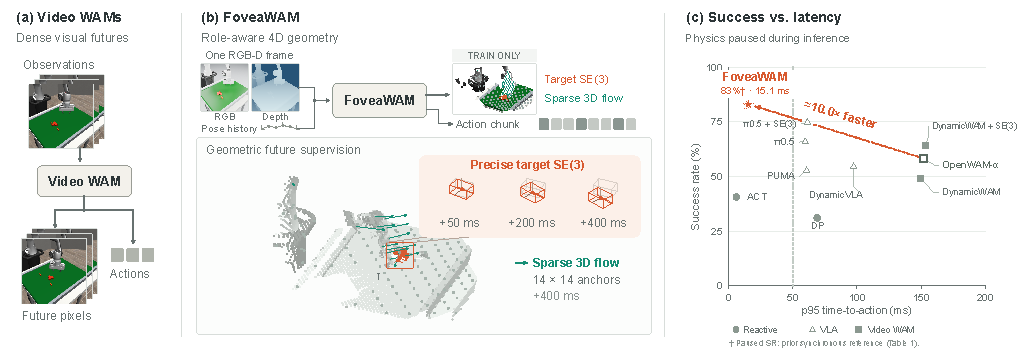
\includegraphics[width=\textwidth]{figures/Fig1/fig1.pdf}
\captionof{figure}{\textbf{\ours 精确地知道目标，粗略地知道场景其余部分。}(a) 一帧 \bench 画面及其训练标签。策略推理期间场景持续运动，因此指令在 $\tau{+}L$ 而非采集时刻 $\tau$ 生效。\ours 在 \cfgHorizons{} 个时域预测目标的度量 SE(3) 位姿（坐标轴），对整个场景只预测 \cfgContextGrid{} 网格上的稀疏 3D 流（箭头；背景上接近零）。两种预测都只用于训练监督，推理时跳过。(b) \bench 上的成功率对 p95 出动作时间，每个方法都计入其自身的实测时延。虚线：50\,ms 控制周期。}
\label{fig:teaser}
\end{center}
